\documentclass[
	ngerman,
	toc=listof, 
	footnotes=multiple, 
	parskip=half, 
	numbers=noendperiod,
	fontsize=12pt
]{scrartcl}

\usepackage[utf8]{inputenc}
\usepackage[T1]{fontenc}

\newcommand{\companyName}{RIS Web- \& Software-Development GmbH \& Co. KG}
\newcommand{\autorName}{Quirin Langer}
\newcommand{\autorEMail}{\href{mailto:langer@ris-development.de}{langer@ris-development.de}}
\newcommand{\autorTel}{+49 941 2000 1250}
\newcommand{\autorPruefNr}{95230}
\newcommand{\projTime}{19.04.2021 - 21.05.2021}
\newcommand{\projectTitle}{Konzeption und Entwicklung einer JTL-Wawi Zusatzsoftware sowie Schnittstelle zur Übersetzung von Texten}
\newcommand{\autorSupervisorName}{Christoph Wagner}
\newcommand{\autorSupervisorEMail}{\href{mailto:wagner@ris-development.de}{wagner@ris-development.de}}
\renewcommand*\pagemark{%
  \usekomafont{pagenumber}{Seite \thepage/\pageref*{LastPage}}%
}
% !TEX root = Projektdokumentation.tex
\usepackage{helvet}
\usepackage{babel}
\usepackage{textcomp}
\usepackage{lmodern}
\usepackage[
    bookmarks,
    bookmarksnumbered,
    bookmarksopen=true,
    bookmarksopenlevel=1,
    colorlinks=false,% diese Farbdefinitionen zeichnen Links im PDF farblich aus
    linkcolor=blue, % einfache interne Verknüpfungen
    anchorcolor=blue,% Ankertext
    citecolor=blue, % Verweise auf Literaturverzeichniseinträge im Text
    filecolor=blue, % Verknüpfungen, die lokale Dateien öffnen
    menucolor=blue, % Acrobat-Menüpunkte
    pdftex,
    plainpages=false, % zur korrekten Erstellung der Bookmarks
    pdfpagelabels=true, % zur korrekten Erstellung der Bookmarks
    hypertexnames=false, % zur korrekten Erstellung der Bookmarks
    linktocpage % Seitenzahlen anstatt Text im Inhaltsverzeichnis verlinken
]{hyperref}
\usepackage{relsize}
\usepackage{setspace}
\usepackage{geometry}
\usepackage{graphicx}
\usepackage{tabularx}
\usepackage{listings}
\usepackage{multirow}
\usepackage{spreadtab}
\usepackage[toc,section=section]{glossaries}
\usepackage[dvipsnames]{xcolor}
\usepackage{dirtree}
\usepackage{lastpage}
\usepackage{eurosym}
\definecolor{hellgelb}{rgb}{1,1,0.9}
\definecolor{colKeys}{rgb}{0,0,1}
\definecolor{colIdentifier}{rgb}{0,0,0}
\definecolor{colComments}{rgb}{0,0.5,0}
\definecolor{colString}{rgb}{1,0,0}
\lstset{
    float=hbp,
	basicstyle=\footnotesize\ttfamily,
    identifierstyle=\color{colIdentifier},
    keywordstyle=\color{colKeys},
    stringstyle=\color{colString},
    commentstyle=\color{colComments},
    backgroundcolor=\color{hellgelb},
    columns=flexible,
    tabsize=2,
    frame=single,
    extendedchars=true,
    showspaces=false,
    showstringspaces=false,
    numbers=left,
    numberstyle=\tiny,
    breaklines=true,
    breakautoindent=true,
	captionpos=b,
}

\lstdefinelanguage{php}{
	sensitive=false,
	morecomment=[l]{/*},
	morestring=[b]",
	morestring=[b]',
	alsodigit={-,*},
	morekeywords={
		abstract,and,array,as,break,case,catch,cfunction,class,clone,const,
		continue,declare,default,do,else,elseif,enddeclare,endfor,endforeach,
		endif,endswitch,endwhile,extends,final,for,foreach,function,global,
		goto,if,implements,interface,instanceof,namespace,new,old_function,or,
		private,protected,public,static,switch,throw,try,use,var,while,xor
		die,echo,empty,exit,eval,include,include_once,isset,list,require,
		require_once,return,print,unset},
}

\usepackage[
    toc, % For the glossaries to appear in the toc.
    numberline, % For the glossaries to have line number references in the toc.
    numberedsection=autolabel, % For the glossaries to have section numbers.
    nonumberlist,
]{glossaries-extra}

\usepackage{pdfpages}
\pdfminorversion=5 

\usepackage{scrlayer-scrpage} 
\makeglossaries{}
% !TEX root = Projektdokumentation.tex
\setlength{\topskip}{\ht\strutbox} 
\geometry{a4paper,left=20mm,right=20mm,top=25mm,bottom=35mm}

\renewcommand{\headfont}{\normalfont} 
\renewcommand*{\othersectionlevelsformat}[3]{
  \makebox[\headingSpace][l]{#3\autodot}
}

\frenchspacing 

\clubpenalty = 10000
\widowpenalty = 10000
\displaywidowpenalty = 10000

\lstset{numbers=left, numberstyle=\tiny, numbersep=5pt, breaklines=true}
\lstset{emph={square}, emphstyle=\color{red}, emph={[2]root,base}, emphstyle={[2]\color{blue}}} 

\renewcommand{\labelenumi}{\arabic{enumi}.}
\renewcommand{\labelenumii}{\arabic{enumi}.\arabic{enumii}}
\renewcommand{\labelenumiii}{\arabic{enumi}.\arabic{enumii}.\arabic{enumiii}}

\definecolor{heading}{rgb}{0.64,0.78,0.86}
\definecolor{odd}{rgb}{0.9,0.9,0.9}

\ihead{\tiny\projectTitle}
\ifoot{\autorName}
\cfoot{}
\ofoot{\pagemark} 
% !TEX root = Projektdokumentation.tex

\newglossaryentry{g:dotnet}{
    name={.NET},
    description={Microsoft .NET; Überbegriff für verschiedene Software-Plattformen zur Ausführung und Entwicklung von Programmen}
}
\newglossaryentry{g:api}{
    name={API},
    description={Application Programming Interface; Eine Programmierschnittstelle zur von Software zu Software}
}
\newglossaryentry{g:bottleneck}{
    name={Bottleneck},
    description={ein Engpass in einem Prozess, in dem die Auslastung besonders hoch ist}
}
\newglossaryentry{g:csv}{
    name={CSV},
    description={Comma seperated values; Dateiformat mit dem meist Tabellen dargestellt werden. Einzelne Spalten werden mit einem Komma [,] getrennt}
}
\newglossaryentry{g:framework}{
    name={Framework},
    description={Bereitstellung eines komponentenbasierten Grundgerüsts}
}
\newglossaryentry{g:gui}{
    name={GUI},
    description={Graphical User Interface; Eine grafische Bedienoberfläche einer Software}
}
\newglossaryentry{g:hashwert}{
    name={Hashwert},
    description={ist eine Art Fingerabdruck eines Datensatzes}
}
\newglossaryentry{g:html}{
    name={HTML},
    description={Hypertext Markup Language; Auszeichnungssprache zur Gliederung von Inhalten. Bildet das Grundgerüst des WWW}
}
\newglossaryentry{g:http}{
    name={HTTP},
    description={Hyper Text Transfer Protokol; Überwiegend in Web-Anwendungen verwendetes zustandsloses Datenübertragungsprotokoll zur Weitergabe von Daten an den Anwender}
}
\newglossaryentry{g:json}{
    name={JSON},
    description={JavaScript Object Notation; Ist ein Programmiersprachenunabhangiges Datenformat, um Daten in einer festgelegten Struktur an den Anwender zu übergeben}
}
\newglossaryentry{g:laravel}{
    name={Laravel},
    description={Framework im Entwurfsmuster Model-View-Controller, dass Bausteine zur Entwicklung von Web-Applikationen bereitstellt}
}
\newglossaryentry{g:middleware}{
    name={Middleware},
    description={ist eine Software die zwischen zwei Anwendungen vermittelt}
}
\newglossaryentry{g:mssql}{
    name={MSSQL},
    description={Microsoft SQL Datenbank}
}
\newglossaryentry{g:mvc}{
    name={MVC},
    description={Model-View-Controller; Ist ein Entwurfsmuster zur Unterteilung der Software-Elemente in Model,View und Controller zur besseren Wiederverwendbarkeit der einzelnen Elemente}
}
\newglossaryentry{g:mysql}{
    name={MySQL},
    description={weitverbreitetes kostenloses Datenbanksystem zur Verwaltung relationaler Datenbanken}
}
\newglossaryentry{g:php}{
    name={PHP},
    description={Hypertext Preprocessing; Weit verbreitete Skript-Sprache, überwiegend in der Web-Entwicklung genutzt}
}
\newglossaryentry{g:rest}{
    name={REST},
    description={Representational State Transfer; Din Architekturstil für die Kommunikation zwischen zwei Softwaresystemen}
}
\newglossaryentry{g:seo}{
    name={SEO},
    description={Search Engine Optimization; Die Optimierung einer Webseite, zur besseren Sichtbarkeit für Suchmaschinen, wie zum Beispiel Google}
}
\newglossaryentry{g:sql}{
    name={SQL},
    description={Structured Query Language}
}
\newglossaryentry{g:storedprocedure}{
    name={Stored-Procedure},
    description={eigenständiger SQL-Befehl der für bestimmte Prozeduren gespeichert wurde}
}
\newglossaryentry{g:url}{
    name={URL},
    description={Uniform Resource Locator; Dient der eindeutigen Adressierung von Dateien und Verzeichnissen und wird hauptsächlich im Internet genutzt}
}
\newglossaryentry{g:win_cron}{
    name={Windows-Aufgabenplanung},
    description={ist eine Windowsfunktion, die es erlaubt Programme zu festgelegten Zeitpunkten zu starten}
}
\newglossaryentry{g:xml}{
    name={XML},
    description={Extensible Markup Language; Wird zur Darstellung und zum Austausch von hierarchisch strukturierterten Daten benutzt}
}
\begin{document}
% !TEX root = Projektdokumentation.tex
\begin{titlepage}
	\centering
	{\huge\bfseries \projectTitle \par}
	\vspace{2.5cm}
	{\Large Bericht zur Projektarbeit zur Erlangung des Abschlusses als\par}
	{\Large\textbf{Fachinformatiker Fachrichtung\\Anwendungsentwicklung}\par}
	\vspace{1.5cm}
	{\Large Arbeit von\par}
    {\Large\textbf{\autorName}\par}
    \vspace{2.5cm}
	\begin{flushleft}
        {\large Betrieb: \companyName{}\par}
        {\large E-Mail: \autorEMail{}\par}
        {\large Telefon: \autorTel{}\par}
        {\large Prüflingsnummer: \autorPruefNr{}\par}
        {\large Ausführungszeit: \projTime{}\par}
        \vspace{1cm}
        {\large Projektbetreuer: \autorSupervisorName{}\par}
        {\large E-Mail: \autorSupervisorEMail{}\par}
	\end{flushleft}
\end{titlepage}


\onehalfspacing 
\phantomsection{}
\pdfbookmark[1]{Inhaltsverzeichnis}{inhalt}
\tableofcontents
\cleardoublepage{}
% !TEX root = Projektdokumentation.tex
\newpage
\section{Einleitung}
\subsection{Projektumfeld}
Meine Ausbildung zum Fachinformatiker für Anwendungsentwicklung absolviere ich in der Firma RIS Web- \& Software-Development GmbH \& Co. KG in Regensburg. 
Der Betrieb beschäftigt derzeit elf Mitarbeiter. 
Als Servicepartner von JTL-Software werden die Warenwirtschaftssoftware (JTL-Wawi) und der E-Commerce-Shop (JTL-Shop) betreut und mit Plugins oder anderen kleinen Softwareerweiterungen zur Abdeckung bestimmter Anforderungen erweitert. 
Für den JTL-Shop werden auch eigene Frontend-Templates umgesetzt. Für die JTL-Wawi zählen Einrichtung, Betreuungen und Schulungen zu den Hauptbereichen. 
Neben der Tätigkeit als Servicepartner werden auch Individuallösungen für Kunden entwickelt und betreut. 
Dazu zählen Entwicklungen von Corporate Designs, Social-Media-Marketing, Neugestaltung/Betreuung von Webseiten, Erstellung von Web-Applikationen und nativer Software.


\subsection{Ist-Analyse}
% Antrag
Unserer Kunden nutzen die E-Commerce-Software JTL-Shop zusammen mit dem Warenwirtschaftsprogramm JTL-Wawi.
Diese werden standardmäßig auf Deutsch installiert, mit der anschließenden Möglichkeit mehrere Sprachen zu nutzen. 
Bei unseren Kunden besteht eine rege Nachfrage nach Übersetzungen in andere Sprachen. 
Derzeit werden diese oft vom Kunden händisch durchgeführt, was bei vielen Artikeln zu sehr viel Arbeitsaufwand führt.
Außerdem müssen bei einer Änderung eines bereits bestehenden Inhalts auch die anderssprachigen Gegenstücke neu übersetzt werden, um Inkonsistenzen zu vermeiden.
%
Im JTL-Ökosystem gibt es zwei für uns relevante Teilbereiche. Zum einen den JTL-Shop, welcher als \gls{g:php}-Web-Applikation betrieben wird und hauptsächlich Fließtexte, aber auch kurze Satzteile in einer Datenbank speichert.
Zum anderen die JTL-Wawi, ein Warenwirtschaftsprogramm, welches auf einem Windows-System agiert, in dem die Artikel, Kategorien sowie Attribute, Beschreibungen und \gls{g:seo}-Inhalte erstellt, und in einer eigenen \gls{g:mssql}-Datenbank gespeichert werden.
Die JTL-Wawi lädt diese Texte außerdem über einen sogenannten Onlineshop-Abgleich in den Shop hoch.
Für beide Softwaresysteme müssen die, gegebenenfalls genutzten, HTML-Tags berücksichtigt werden.

\subsection{Soll-Zustand}
\label{sec:soll}
Zu Entwickeln sind daher ein JTL-Shop Plugin, eine Zusatzsoftware zur JTL-Wawi sowie eine Schnittstelle für uns. 
Diese Schnittstelle wird die Kommunikation mit dem tatsächlichen Übersetzungs-Service übernehmen.
Dabei soll sie zu übersetzende Texte entgegennehmen, an einen Übersetzungs-Dienst übertragen und die übersetzten Inhalte zurück liefern, sowie Nutzungsmetriken pro Kunde erfassen, zur Erhebung von Übersetzungsgebühren.

Meine Aufgaben werden die Entwicklung und Konzeption der Schnittstellen-Software und die Umsetzung der Zusatzsoftware auf dem Windowssystem sein.
Damit soll die Übersetzung automatisiert an einen Drittanbieter ausgelagert werden, um den Arbeitsaufwand und mögliche Fehler zu minimieren.

\subsection{Lösungsansätze}
\label{sec:solutions}
Bei Automatisierungen in einem großen Ausmaß, ist es wichtig den richtigen Ausführungszeitpunkt zu wählen. 
Dabei gilt es verschiedene Möglichkeiten abzuwägen, beispielsweise feste Uhrzeiten, oder stündliche Intervalle sowie das Aufrufen, wenn es einen neuen übersetzbaren Wert gibt. 
Eine feste Uhrzeit bei all unseren Kunden würde zu extremer Belastung der Schnittstelle führen, welche als API umgesetzt wird.
Mehrmals täglich zu übersetzen, bietet den großen Vorteil, dass Änderungen schneller übernommen werden können und die Auslastung der \gls{g:api} würde sich besser verteilen. 
Zusätzlich wäre ein Option eines manuellen Anstoßes sicherlich von Vorteil.

Eine weitere Unklarheit, die vor der Umsetzung der Zusatzsoftware genauer betrachtet werden sollte, ist die Art der Datenbankzugriffe auf die Datenbank der JTL-Wawi.
Es gibt zwei Arten auf die \gls{g:mssql}-Datenbank zuzugreifen, direkt über \gls{g:sql} oder über die von JTL bereitgestellte Software JTL-Ameise. 
Sie ermöglicht einen überwachten und einwandfreien lesenden und schreibenden Zugriff auf die Datenbank. 
Dabei können große Mengen an Anpassungen, der gleichen Art, in einem Durchlauf durchgeführt werden, was für die Übersetzungen optimal ist.
Diese Software ist jedoch erfahrungsgemäß sehr langsam (ein Export mit etwa 50.000 Artikeln braucht je nach Server etwa 4 Stunden).
Der direkte Zugriff auf die Datenbank mit Hilfe von \gls{g:sql} ist deutlich schneller, 
jedoch sprechen die stetigen Datenbank-Schema-Veränderungen bei Updates, sowie fehlende \gls{g:storedprocedure}s dagegen.
Kleinste Fehler können zu Inkonsistenzen in den Tabellen oder Datenverlust führen.
Da die Datenbank mit sehr sensiblen Kundendaten arbeitet und die Zugriffe nicht für jede Wawi-Version exakt gleich sind, fällt die Wahl auf JTL-A

Die Auswahl der Technologien und Systeme für die (REST-)\gls{g:api} ist groß, daher es gibt hier vor allem Entscheidungskriterien, der Wartbarkeit und Erweiterbarkeit. 
In meinem Betrieb ist \gls{g:php} allgegenwärtig und daher im Vergleich zu JavaScript deutlich wartbarer für alle Kollegen. 
Die Entscheidung, die \gls{g:api} in \gls{g:php} zu programmieren, fiel daher recht schnell und einfach.

Für die Übersetzungssoftware wurden verschiedene Anbieter wie Amazon Translate, Google Translate, Microsoft Translator und DeepL Translator getestet. 
Dabei konnten die namenhaften Dienstleister leider entweder qualitativ nicht mithalten, oder bieten keine \gls{g:api}, die aufgerufen werden kann. 
Daher soll der Übersetzungsdienst von DeepL benutzt werden.
Er bietet nicht nur sehr gute Übersetzungen, sondern außerdem auch eine Vielzahl an verschiedenen Ein-/ und Ausgangssprachen sowie die Option, HTML zu berücksichtigen. 
Die Nutzung des Services via \gls{g:api} ist zwar nicht kostenlos, jedoch wird für die sehr gute Übersetzungsqualität nur ein kleiner Betrag pro Zeichen fällig.


\subsection{Technologieplattform}

Die Nutzung eines \gls{g:framework} wie \gls{g:laravel} bietet sich bei der Arbeit mit \gls{g:php} zusätzlich an, da die Entwicklung vereinfacht und beschleunigt werden kann. 
Dank der hervorragenden Dokumentation hat sich \gls{g:laravel} in der Vergangenheit als sicher, schnell, zuverlässig und auf Grund des Model-View-Controller-Entwurfsmusters (\gls{g:mvc}) auch als sehr übersichtlich herausgestellt. 
Dabei repräsentieren \emph{Models} Daten, die von einem \emph{Controller} verarbeitet werden und dann mit Hilfe einer \emph{View} als (optische) Ausgabe dargestellt werden können.
\gls{g:laravel} bietet außerdem standardmäßig eine MySQL-Unterstützung, welche für das Projekt genutzt werden wird.

Da die JTL-Wawi das Microsoft .NET Framework voraussetzt, kann auch eine C\#-Applikation problemlos ausgeführt werden. 
Daher bietet sich C\# als Programmiersprache an und wird im Projekt für die Umsetzung der Zusatzsoftware benutzt. 

Für die Datenbankzugriffe wird das von JTL bereitgestellte Programm JTL-Ameise verwendet, da es erlaubt alle Datenbanktabellen der JTL-Wawi zu ex-/ bzw. importieren. 
Das Programm arbeitet mit \gls{g:csv}-Dateien, was eine angenehme Dateiverarbeitung ermöglicht und mit C\# leicht verarbeitet werden kann.

Zuletzt gilt es den Dienst zu erwähnen, welcher für die Übersetzung genutzt wird. 
DeepL hat sich als eine sehr hochwertige Übersetzungssoftware entpuppt, daher wird sie in diesem Projekt ihre Anwendung finden.

Da bereits die DeepL-\gls{g:api} über das \gls{g:json}-Format kommuniziert, bietet sich dieses auch für die \gls{g:middleware} an.
\newpage
\section{Entwurfsphase}
\subsection{Schnittstelle}

\subsubsection{Datenbankmodell}
Da die \gls{g:api} Anfragen empfängt und diese den richtigen Kunden für die Abrechnung zuordnen soll, braucht es zwei Tabellen. 
Eine für den Kunden ('customers') und eine für dessen Übersetzungsanfragen ('translation\_requests').
In 'customers' wird der Kunde und sein \gls{g:api}-Schlüssel zur Identifikation gespeichert, 
während in 'translation\_requests' der Inhalt, dessen Zeichenlänge, ein Zeitstempel so wie die Verknüpfung zum Kunden hinterlegt werden soll.
Für die Abrechnung muss eine Übersetzungsanfrage immer genau einem Kunden zugewiesen werden können (siehe Anhang \ref{sec:erd-api}).

\subsubsection{Aufbau}
\gls{g:rest}-\gls{g:api} steht für \emph{Representational State Transfer Application Programming Interface}. 
Der Hauptanwendungsbereich dieser Schnittstellen sind Web-Applikationen, welche mittels \gls{g:http} Anfragen, wie \texttt{GET}, \texttt{PUT}, \texttt{POST} oder \texttt{DELETE}, Daten zwischen Softwaresystemen austauschen können.
Dabei werden in diesem Fall die Datenpakete im \gls{g:json}-Format übertragen, um eine standardisierte Strukturierung zu ermöglichen.

Eine \gls{g:api} hat oft mehrere Endpunkte, welche jeweils mit unterschiedlichen \gls{g:http}-Methoden genutzt werden können (siehe Anhang \ref{sec:table_http_request}).
Die \gls{g:api} wird mit dem \gls{g:php}-\gls{g:framework} \gls{g:laravel} erstellt. 
Dabei folgt es dem \gls{g:mvc}-Entwurfsmuster, welches sich durch die Trennung der Anwendungslogik von Darstellung und Benutzerinteraktionen auszeichnet.

Die \emph{Models} der \gls{g:api} beziehen sich auf die beiden Datenbanktabellen (siehe Anhang \ref{sec:table_tranlation_request} und \ref{sec:table_customers}), und können aus einer Tabellenzeile jeweils ein Objekt formen.
Der \emph{View} gibt übersetzte Inhalte in Form eines \gls{g:json}-Objekts zurück.

Außerdem wird ein \emph{Controller} für die Verarbeitung der \emph{Requests} benutzt.
Er wird Texte empfangen, eine Übersetzungsanfrage an DeepL stellen und anschließend den übersetzen Wert zurückgeben.
Die gesamte Verarbeitungslogik passiert ebenfalls im Controller.

\subsection{Zusatzsoftware}
\subsubsection{Datenbankmodell}
Um einen vorliegenden Datensatz nicht zu übersetzen, obwohl dieser schon einmal übersetzt wurde, muss abgespeichert sein, dass es bereits eine Übersetzung in die jeweilige Sprache gibt. 
Ansonsten entstehen Kosten und Zeitaufwand/Auslastung am Server, die man auch vermeiden kann.

Um mögliche Änderungen in einem Text erkennen zu können, muss ein Indikator entworfen werden, der schnell auslesbar ist und wenn möglich Versionen, anhand der Länge oder eines Zeitstempels erkennt.
Dieser wird anschließend, zusammen mit einem eindeutigen Identifikator des übersetzten Textes in einer Datenbanktabelle gespeichert (siehe Anhang \ref{sec:erd-csharp}).

\subsubsection{Aufbau}
Die Zusatzsoftware wird in C\# und damit auch objektorientiert programmiert. 
Sie wird die Texte, mit Hilfe der JTL-Ameise, aus der Datenbank der JTL-Wawi auslesen und anschließend diese gelesenen Werte an die \gls{g:api} schicken.
Die Antworten des Übersetzungsdienstes werden dann als neue Datensätze in eine, für die JTL-Ameise lesbare \gls{g:csv}-Datei, geschrieben und importiert.

Um die Verarbeitungslogik von den Im-/ Exporten sowie den \gls{g:api}-Aufrufen zu trennen, werden verschiedene Klassen entworfen.
Dabei werden die Kommunikationswege zwischen der Zusatzsoftware und der JTL-Ameise bzw. \gls{g:api} in jeweils eine eigene Klasse gespalten. 
Außerdem soll die Verarbeitung und Aufbereitung der \gls{g:csv}-Dateien ebenso vom restlichen Programmcode separiert werden. 

\newpage
\section{Implementierung}
\subsection{Schnittstelle}
\subsubsection{Datenbanktabellen/Migrations}
Eine Datenbank-Tabelle kann in Laravel mit Hilfe von \emph{Migrations} erzeugt und manipuliert werden. 
Für jede Tabelle wird also eine eigene Klasse erstellt, die von der \emph{Migration}-Klasse erbt.
Außerdem werden in jeder solchen Klasse zwei Methoden implementiert, welche für strukturelle Änderungen in der Datenbank sorgen können. 
Die \texttt{up()} Methode setzt die Änderungen um, während die \texttt{down()} Methode die Änderungen wieder Rückgängig macht (siehe Anhang \ref{sec:migration_translation_request}).
So entsteht eine Art Versionierungsprotokoll.

Da die \gls{g:api} derzeit noch keine \gls{g:gui} besitzt, wurde intern beschlossen die Ausgabe der Nutzungsdaten der Kunden über einen \gls{g:sql}-Befehl auszulesen. 
So werden die Metriken derzeit monatlich über eine Datenbankverwaltungssoftware ausgelesen. 
Im Anhang \ref{sec:sql_data} wird der Befehl für den Monat Mai aufgezeigt.

\subsubsection{Entitätstypen/Models}
Für jede Datenbanktabelle wird außerdem eine Klasse benötigt, welche man als \emph{Model} bezeichnet.
Im Fall dieser \gls{g:api} gibt es also die \emph{Models} \texttt{Customer} und \texttt{TranslationRequest}.
Diese beinhalten nicht nur die Attribute, die die Tabellenspalten repräsentieren, sondern ggf. auch kleinere Codeteile, beim Schreiben eines Datensatzes aufgerufen werden.
So kann beispielsweise beim Setzen des Attributs \texttt{content} direkt die Länge der Zeichenkette berechnet und in einer weiteren Variablen gespeichert werden (siehe Anhang \ref{sec:model_translation_request} Zeile 24ff.).
Außerdem sind in der Klasse \texttt{Model} die Funktionalitäten für die Datenbankoperationen, wie zum Beispiel \texttt{save()}, \texttt{update()} oder \texttt{delete()} verankert.

\subsubsection{Controller}
Die verschiedenen \emph{Routen} werden von einer Methode im jeweiligen \emph{Controller} bedient. 

\texttt{POST: /api/translation\_request/?[params]}


Die \texttt{POST}-Anfrage an diese \emph{Route} wird vom \texttt{TranslationRequestController} mit der Methode \texttt{store()} bedient (siehe Anhang \ref{sec:controller_translation_request}).
Dort werden zu Beginn die Daten der Anfrage validiert. 
Sollte dies fehlschlagen, wird automatisch ein Fehler zurückgegeben, ansonsten wird eine Verknüpfung zum Kunden, anhand des \gls{g:api}-Keys, hergestellt. 
Es wird eine neue Instanz des \texttt{DeeplService}s erstellt und die \texttt{translate()} Methode mit dem Text als Übergabeparameter aufgerufen.
Nachdem die Antwort mit dem übersetzten Text angekommen ist, kann dieser zurückgegeben werden.

\subsubsection{Services}
Die Kommunikation mit der \gls{g:api} von DeepL wird in einen \emph{Service} gespalten, um die Verarbeitungslogiken sinnvoll voneinander zu Trennen.
Die \texttt{translate()} Methode (siehe Anhang \ref{sec:deeplservice}) liest eine Konfigurationsdatei aus, in der sowohl die DeepL-\gls{g:api}-\gls{g:url} als auch ein \gls{g:api}-Token für die Authentifizierung liegt.
Im Anschluss wird eine \gls{g:http}-Anfrage an die DeepL-\gls{g:api}, aus den übergebenen Daten formuliert.
Dazu gehören ein Header, welcher einen \texttt{user-agent} verlangt, sowie der tatsächliche Inhalt, welcher aus einem Parameterobjekt besteht.
Das Ergebnis ist der übersetzte Inhalt oder ein Fehler, welcher direkt weiter and den \emph{Controller} zurückgegeben wird.


\subsection{Zusatzsoftware}

\subsubsection{Konfiguration}
Die in \ref{sec:solutions} angesprochenen langen Wartezeiten können mit Hilfe einer Filterung deutlich verkürzt werden. 
Die JTL-Wawi bietet Automatisierungsprozesse mit denen Artikel beim Verändern eine Markierung bekommen können, so werden die Exporte um ein vielfaches kleiner und somit schneller.

Um \gls{g:csv}-Dateien über die JTL-Ameise zu im-/exportieren, müssen vorher Im-/ und Exportvorlagen erstellt werden.
Das passiert händisch über die \gls{g:gui} der JTL-Ameise (siehe Anhang \ref{sec:ameise}).

Außerdem muss eine Konfigurationsdatei mit den Zugangsdaten zur JTL-Wawi Datenbank befüllt werden (siehe Anhang \ref{sec:config}).

\subsubsection{SqlHelper Klasse}
Zu Beginn des Programmstarts wird, mit Hilfe der Konfigurationsdatei, eine Verbindung zur JTL-Wawi Datenbank hergestellt und falls noch nicht geschehen, zwei neue Tabellen angelegt.
Dazu wird die \texttt{SqlHelper} Klasse aufgerufen, welche eine \texttt{execute()} Methode zur Verfügung stellt, die einen übergebenen SQL-Befehl ausführen kann (siehe Anhang \ref{sec:sql_helper}). 
In den Tabellen wird gespeichert, welche Texte bereits übersetzt wurden.
Um eine Prüfsumme der übersetzten Datensätze zu erhalten, wird ein \gls{g:hashwert} des Originaltexts gebildet und zusammen mit einem, aus zwei Elementen bestehenden, Identifikator gespeichert (siehe Anhang \ref{sec:table_hash}). 
Da ein Text in mehrere Sprachen übersetzt werden kann, entsteht eine '1 zu n' Beziehung, welche mit einer weiteren Tabelle aufgelöst wird (siehe Anhang \ref{sec:table_hash_language}).

\subsubsection{AntHelper Klasse}
Sind die Tabellen vorhanden wird im nächsten Schritt die JTL-Ameise mit den vorher erstellten Exportvorlagen aufgerufen.
Dafür wird ein Objekt der Klasse \texttt{AntHelper} erstellt und die \texttt{export()} Methode aufgerufen (siehe Anhang \ref{sec:api_helper}).
Wenn die Exporte vollständig abgearbeitet wurden, sind im dafür vorgesehenen Verzeichnis die \gls{g:csv}-Dateien mit den zu übersetzenden Daten gespeichert.
Die Klasse bietet außerdem eine Methode \texttt{import()} um später übersetzte Inhalte wieder in die JTL-Wawi Datenbank zu schreiben, dazu wird eine \gls{g:csv}-Datei und ein passendes Importformat benötigt.

\subsubsection{CsvHelper und ApiHelper Klasse}
Zum Verarbeiten der \gls{g:csv}-Dateien wird eine .NET-Bibliothek namens \texttt{CsvHelper} verwendet. 
Sie ermöglicht es, die zu übersetzenden Texte, Feld für Feld aus der \gls{g:csv}-Datei auszulesen.
Die gelesenen Datensätze werden anschließend an ein neues Objekt der Klasse \texttt{ApiHelper} als Übergabeparameter weitergegeben, um eine Übersetzung anzustoßen.
Wird der Datensatz erfolgreich übersetzt, so wird der \gls{g:hashwert} davon in der Tabelle \texttt{hash} gespeichert, und je nach Sprachen entsprechende Verweise in der Tabelle \texttt{hash\_language} gespeichert.
Anschließend wird erneut das Objekt der \texttt{CsvHelper} Bibliothek genutzt, um eine \gls{g:csv}-Datei für den Import zu schreiben.

Nach erfolgreichem Schreiben der Import-Datei wird der \texttt{AntHelper} erneut aufgerufen, diesmal mit der Methode \texttt{import()}.
Der Vorgang wird mittels der \gls{g:win_cron} in regelmäßigen Abständen wiederholt, kann aber auch manuell gestartet werden.

\newpage
\section{Testphase}
\subsection{Schnittstelle}
Die Datenbankanbindung wurde bereits während der Entwicklung getestet und mit Hilfe eines MySQL-Plugins direkt in der Entwicklungsumgebung überprüft.
Da die \gls{g:laravel}-Controller mit Hilfe der \emph{Models} bereits in der Lage sind, die Datenbank zu beschreiben, wenn ein passendes \emph{Model} vorliegt, mussten hier keine weiteren Tests gemacht werden.
Somit wurden die Datenbanktabellen lediglich auf ihre Richtigkeit sichtgeprüft. 

Die Schnittstelle dient als \gls{g:middleware} und gibt Fehler, die bei der Verbindung mit der DeepL-\gls{g:api} auftreten, direkt weiter an den Endnutzer.
Bei Fehlern in der Schnittstelle selbst werden Statuscodes in die Datenbank geschrieben.

Ansonsten wurden, mittels Testanfragen, vor allem überprüft, dass keine Routen für den Endnutzer verfügbar sind, mit denen Daten aus der Datenbank gelesen werden können.

Auch die Validierung in der \texttt{store()} Methode des \texttt{TranslationRequestController} wurde ausgiebig überprüft, indem verschiedene fehlerhafte Parameter an die Route übersendet wurden. 

\subsection{Zusatzsoftware}
Für die Zusatzsoftware zur JTL-Wawi wurden vor allem die einzelnen Klassen an sich getestet. 

Zuerst muss das Programm eine problemfreie Verbindung mit der Datenbank herstellen können, um auch schnell und zuverlässig eine Überprüfung durchführen zu können.

Anschließend wurde überprüft, ob der Aufruf der JTL-Ameise korrekt funktioniert. 
Das kann lediglich von einem Menschen kontrolliert werden, indem die CSV-Datei auf ihre Integrität sichtgeprüft wird.

Um die Anbindung an die \gls{g:api} zu testen, wurde im Controller ein \texttt{api\_key} hinterlegt, für den kein Übersetzungsprozess angestoßen wird, 
sondern lediglich das Kürzel der Zielsprache mit dem Ausgangstext in Klammern ausgegeben wird (siehe Anhang \ref{sec:testing_api}).
So können größere Tests durchgeführt werden, ohne Kosten zu verursachen, solange der Test-\gls{g:api}-Schlüssel in der Anfrage angegeben wird.
\newpage
\section{Schluss}
\subsection{Soll-Ist-Vergleich}
\begin{center}
    \begin{tabular}{ |l|r|r|r| }
        \hline
        \textbf{Projektphasen} & \textbf{Soll-Zeit [h]} & \textbf{Ist-Zeit [h]} & \textbf{Differenz [h]} \\
        \hline  
        \textbf{Projektplanung} & & & \\
        \hspace{0.65cm} Ist-Analyse & 2 & 2 & 0 \\
        \hspace{0.65cm} Soll-Konzept & 2 & 2 & 0 \\
        \hspace{0.65cm} Lösungsansätze vergleichen & 2 & 2 & 0 \\
        \hline  
        \textbf{Entwurf} & & & \\
        \hspace{0.65cm} Datenbankmodell Schnittstelle & 1 & 1 & 0\\
        \hspace{0.65cm} Datenbankmodell Zusatzsoftware & 2 & 2 & 0 \\
        \hspace{0.65cm} Aufbau Schnittstelle & 4 & 3 & \textcolor{Green}{-1}\\
        \hspace{0.65cm} Aufbau Zusatzsoftware & 4 & 6 & \textcolor{red}{+2} \\
        \hline  
        \textbf{Implementierung} & & & \\
        \hspace{0.65cm} \textbf{Schnittstelle} & & & \\
        \hspace{1.3cm} Erstellen der Datenbank & 5 & 4 & \textcolor{Green}{-1} \\
        \hspace{1.3cm} Logik zur Verarbeitung & 10 & 9 & \textcolor{Green}{-1} \\
        \hspace{1.3cm} Ausgabe der Metriken & 3 & 2 & \textcolor{Green}{-1} \\
        \hline  
        \hspace{0.65cm} \textbf{Zusatzsoftware} & & & \\
        \hspace{1.3cm} Datenbankintegration & 4 & 4 & 0\\
        \hspace{1.3cm} Erfassung von übersetzten Inhalten & 2 & 3 & \textcolor{red}{+1} \\
        \hspace{1.3cm} Im- und Exportformate & 5 & 6 & \textcolor{red}{+1}\\
        \hspace{1.3cm} Verarbeitung der Daten & 5 & 6 & \textcolor{red}{+1}\\
        \hline  
        \textbf{Testen} & & & \\
        \hspace{0.65cm} Testen der Schnittstelle & 3 & 3 & 0\\
        \hspace{0.65cm} Testen der Zusatzsoftware & 5 & 4 & \textcolor{Green}{-1} \\
        \hline  
        \textbf{Projektabschluss} & & & \\
        \hspace{0.65cm} Soll-Ist-Vergleich & 1 & 1 & 0\\
        \hspace{0.65cm} Dokumentation & 7 & 7 & 0\\
        \hspace{0.65cm} Abnahme & 1 & 1 & 0\\
        \hspace{0.65cm} Wirtschaftlichkeitsanalyse & 1 & 1 & 0\\
        \hline
        Gesamtstunden: & 70 & 70 & 0\\
        \hline
    \end{tabular}
\end{center}
Der Aufbau der Schnittstelle konnte durch die Verwendung von \gls{g:laravel} deutlich schneller als erwartet festgelegt werden. 
Ebenso wurde durch die vorgegebene Struktur von \gls{g:laravel} viel Zeit bei der Erstellung von Datenbanken und Klassen eingespart.

Dafür war die Handhabung der JTL-Wawi Datenbankzugriffe ein größeres Problem als ursprünglich geschätzt. 
Auch die Implementierung dauerte dadurch etwas länger als zunächst erwartet. 

\subsection{Dokumentation und Abnahme}
Es wurde eine \gls{g:api}-Dokumentation (siehe \ref{sec:api_documentation}.) für Endnutzer, sowie eine Installationsanleitung zur Zusatzsoftware (siehe \ref{sec:tool_documentation}.) erstellt. 
Die Software wurde anschließend zum Code-Review an ein Entwicklerteam abgegeben.

\subsection{Wirtschaftlichkeitsanalyse}
\subsubsection{Kosten}
Die Entwicklung des Projekts beläuft sich auf 70h. 
Hinzu kommen 70h die für die Entwicklung eines JTL-Shop-Plugins von einem Kollegen, wie in \ref{sec:soll} beschrieben.

Aus buchhalterischer Sicht fallen für einen Auszubildenden pro Stunde etwa 20€ brutto an Kosten an. Außerdem ist noch ein Gemeinkostenzuschlagsatz von etwa 10\% zu verrechnen. 
Somit betragen die gesamten Entwicklungskosten \( 3080\text{€} = ((70\text{h} + 70\text{h}) \cdot 20\text{€} ) + 10\%   \).

Die Einrichtung pro Kunde nimmt etwa 4h in Anspruch und muss ebenfalls mit Kosten von 20€/h berücksichtigt werden.

Die Kosten für die Übersetzung eines Shops ist abhängig von der Anzahl der zu übersetzenden Zeichen. 
Des weiteren sind die laufenden Kosten für Änderungen und neue Texte nur schwer einzuschätzen und stark abhängig von der Schnelllebigkeit des Sortiments. 

DeepL berechnet für 1.000.000 Zeichen exakt 20€ und eine monatliche Grundgebühr von 5€. 
Das bedeutet, dass pro Shop und pro Sprache initial mit etwa 60€ Kosten zu rechnen sind, und monatlich etwa 3€ anfallen.

\footnotetext[1]{Annahme: Ein Shop enthält 3 Mio. Zeichen sowie eine monatliche Erneuerungsrate von 5\%.}
\footnotetext[2]{Wird nur einmalig fällig. Bei weiteren Kunden muss der Betrag nicht erneut bezahlt werden.}

\paragraph{Beispiel für einen Kunden:}
\begin{center}
    \begin{tabular}{l r}
        \textbf{Kosten einmalig} & \textbf{Betrag} \\
        % 1. Entwicklung & 3080€ \\
        1. Einrichtung & 80€ \\
        2. initiale Übersetzung\footnotemark[1] & 60€ \\
        \hline
        Gesamt: & 140€ \\
    \end{tabular}
    \hspace{2.9cm}
    \begin{tabular}{l r}
        \textbf{Kosten monatlich} & \textbf{Betrag} \\
        % 1. Server/Domain & 5€ \\
        1. Bereitstellungspauschale\footnotemark[2] & 5€\\
        2. monatl. Zeichenmenge\footnotemark[1] & 3€\\
        \hline
        Gesamt: & 8€ \\
    \end{tabular}
\end{center}

\subsubsection{Einnahmen}
Das Abrechnungskonzept von DeepL bleibt gegenüber dem Kunden unverändert und besteht aus einer Bereitstellungspauschale, 
sowie eines Tarifs für die Anzahl der übersetzten Zeichen.
Die Bereitstellungspauschale soll pro Kunde im Jahr etwa 10\% der Entwicklungskosten betragen.
\[
    \frac{3080\text{€} \cdot 0.1}{12} = 25.66\text{€} \approx 25\text{€} / \text{Monat}
\]

Hinzukommend wird eine Einrichtungspauschale von 400€ einmalig fällig.
Außerdem werden die Übersetzungskosten mit einer Gewinnmarge von 100\% an den Kunden weitergegeben, daher verdoppeln sich alle Übersetzungskosten.

\begin{center}
        \begin{tabular}{ l r }
            \textbf{Kosten einmalig} & \textbf{Betrag} \\
            1. Einrichtungspauschale & 400€ \\
            2. initiale Übersetzung\footnotemark[1] & 120€ \\
            \hline
            Gesamt: & 520€ \\
        \end{tabular}
        \hspace{2.9cm}
        \begin{tabular}{l r}
            \textbf{Kosten monatlich} & \textbf{Betrag} \\
            1. Bereitstellungspauschale & 25€ \\
            2. monatl. Zeichenmenge\footnotemark[1] & 6€\\
            \hline
            Gesamt: & 31€ \\
        \end{tabular}
\end{center}
\footnotetext[1]{Annahme: Ein Shop enthält 3 Mio. Zeichen sowie eine monatliche Erneuerungsrate von 5\%.}


\subsubsection{Fazit}
Bei der Einrichtung ergibt sich somit ein Gewinn von 380€, sowie ein monatlicher Gewinn von etwa 18€ pro Kunde.

Somit kann berechnet werden, wie viel anschließend noch bis zu Amortisierung fehlt:
\[
    3080\text{€} - (3 \cdot 380\text{€}) = 1940\text{€}
\]

Berechnung der Amortisierung mit 3 Kunden anhand der laufenden Kosten:
\[
    \frac{1940\text{€}}{3 \cdot 18\text{€}} = 35.93 \text{ Monate} \approx 36 \text{ Monate}
\]

Mit drei Kunden und durchschnittlichen Nutzungswerten würde sich das Projekt nach 3 Jahren amortisieren. 
Das ist eine sehr weitsichtige Investition und damit sehr risikoreich.
Nach sorgfältiger Rücksprache mit den drei auftraggebenden Kunden wurde beschlossen, die Entwicklungskosten zu gleichen Teilen auf sie aufzuteilen.
Somit ist das Projekt von der Fertigstellung an amortisiert. Da die laufenden Kosten deutlich unter den laufenden Einnahmen liegen, 
können die Gewinne in die Instandhaltung, Wartung und Erweiterung der Software reinvestiert werden.
 

\subsection{Ausblick}
Das Projekt war erfolgreich und wird vorraussichtlich mehr als nur die auftraggebenden Kunden erreichen.

Es bieten sich noch einige Erweiterungsmöglichkeiten an, welche nicht mehr im Rahmen des Projekts abwickelbar waren. 
Beispielsweise eine GUI für das Auslesen und Beschreiben der \gls{g:api}-Datenbanken, um leichter Kunden hinzuzufügen oder deren Nutzungsdaten auszulesen.
Auch eine Automatisierung der monatlichen Abrechnung wäre denkbar und sinnvoll.

Je mehr Kunden das Produkt erhalten, desto wichtiger wird die Robustheit der \gls{g:api}, so könnte es in Zukunft relevant sein, ein mögliches \gls{g:bottleneck} in der \gls{g:api} zu verhindern.
\newpage
\printglossaries{}
\newpage
% !TEX root = Projektdokumentation.tex
% \renewcommand\thesection{\Alph{section}}
\renewcommand\thesubsection{\Alph{subsection}}
\section{Anhang}
\subsection{Schnittstelle: ER-Diagramm}
\label{sec:erd-api}
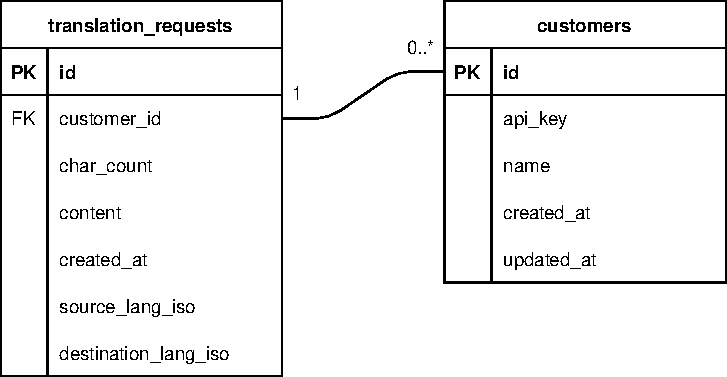
\includegraphics[width=15cm]{./img/ERD-API.pdf}

\subsection{Liste der HTTP-Endpunkte}
\label{sec:table_http_request}
\begin{tabular}{ |l|l|l| }
	\hline
	Methode & URI & Beschreibung \\ 
	\hline
	GET & api/ruok  & Gibt den aktuellen Status der API zurück \\  
	GET & api/translation\_request  & Zeigt alle gespeicherte Datensätze \\  
	POST & api/translation\_request & Schreibt einen Datensatz \\
	GET & api/translation\_request/\{ id \}  & Zeigt einen Datensatz \\  
	PUT & api/translation\_request/\{ id \} & Ändert einen Datensatz \\
	DELETE & api/translation\_request/\{ id \} & Löscht einen Datensatz \\
	\hline
\end{tabular}

\subsection{Tabelle 'translation\_requests'}
\label{sec:table_tranlation_request}
\begin{center}
\begin{tabular}{ |l|l|l|l|l|l|l|l| }
    \hline
    ID & content & source & destination & count & customer\_id  & status & created\_at\\ 
    \hline
    \dots & \dots & \dots & \dots & \dots & \dots & \dots & \dots\\  
    186 & Tisch & DE & EN & 5 & 1 & 200 & 2021-04-29 12:44:48 \\  
    187 & Straße & DE & EN & 7 & 1 & 200 & 2021-04-29 12:45:38 \\  
    188 & Maske & DE & EN & 5 & 2 & 200 & 2021-04-29 12:46:30 \\  
    189 & Uhr & DE & EN & 3 & 1 & 200 & 2021-04-29 12:55:16 \\  
    \dots & \dots & \dots & \dots & \dots & \dots & \dots & \dots\\  
    \hline
\end{tabular}
\end{center}

\subsection{Tabelle 'customers'}
\label{sec:table_customers}

\begin{center}
\begin{tabular}{ |l|l|l|l|l| }
    \hline
    ID & api\_key & name & created\_at & updated\_at \\ 
    \hline
    1 & d6c117cfa61375\dots & langer@[\dots].de & 2021-04-29 12:47:56 & 2021-04-29 12:47:56\\  
    2 & b6f8d434a847fb\dots & birnthaler@[\dots].de & 2021-04-29 12:47:56 & 2021-04-29 12:47:56\\  
    \dots & \dots & \dots & \dots & \dots\\  
    \hline
\end{tabular}
\end{center}

\subsection{Zusatzsoftware: ER-Diagramm}
\label{sec:erd-csharp}
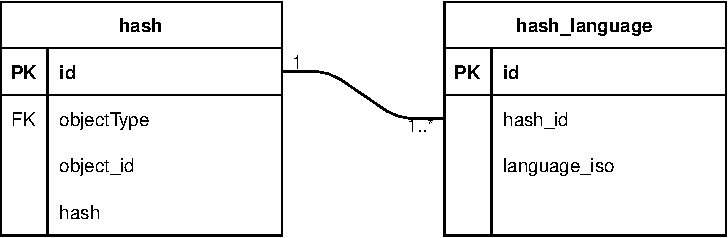
\includegraphics[width=15cm]{./img/ERD-Cscharp.pdf}


\newpage
\subsection{Migration 'translation\_request'}
\label{sec:migration_translation_request}
\begin{lstlisting}[language=php]
<?php

use Illuminate\Database\Migrations\Migration;
use Illuminate\Database\Schema\Blueprint;
use Illuminate\Support\Facades\Schema;

class CreateTranslationRequestsTable extends Migration
{
	// 
	// Run the migrations.
	// @return void
	// 
	public function up()
	{
		Schema::create('translation_requests', function (Blueprint $table) {
			$table->id();

			$table->longText('content');

			$table->string('source_language_iso', 2);
			$table->string('destination_language_iso', 2);

			$table->bigInteger('char_count');
			$table->integer('status');
			$table->foreignId('customer_id')->constrained('customers');

			$table->timestamps();
		});
	}

	// 
	// Reverse the migrations.
	// @return void
	// 
	public function down()
	{
		Schema::dropIfExists('translation_requests');
	}
}
\end{lstlisting}

\newpage
\subsection{Auslesen der Metriken}
\label{sec:sql_data}
\begin{lstlisting}[language=sql]
SELECT  c.name as "Kunde", SUM(char_count) as "Anzahl der Zeichen"
FROM translation_requests as r
JOIN customers c ON r.customer_id = c.id
WHERE r.created_at 
BETWEEN "2021-05-01 00:00:00" AND "2021-05-31 23:59:59"
GROUP BY c.name
\end{lstlisting}

Ausgabe 

\begin{tabular}{|l|r|}
    \hline
    Kunde & Anzahl der Zeichen\\
    \hline
    langer@ris-development.de & 256187\\
    birnthaler@ris-development.de & 65536\\
    \hline
\end{tabular}

\subsection{Model 'TranslationRequest'}
\label{sec:model_translation_request}
\begin{lstlisting}[language=php]
<?php
namespace App\Models;

use Illuminate\Database\Eloquent\Factories\HasFactory;
use Illuminate\Database\Eloquent\Model;

class TranslationRequest extends Model{
    use HasFactory;
    protected $fillable = [
        'content',
        'source_language_iso',
        'destination_language_iso',
        'char_count',
        'status',
        'customer_id',
    ];

    protected $attributes = [
        'char_count' => 0,
        'status' => 1,
    ];
    
    public function setContentAttribute($value){
        $this->attributes['content'] = $value;
        $this->attributes['char_count'] = strlen($value);
    }
}
\end{lstlisting}

\newpage
\subsection{Controller 'TranslationRequest'}
\label{sec:controller_translation_request}
\begin{lstlisting}[language=php]

class TranslationRequestController extends Controller{

    public function store(Request $request){

        $data = $request->validate([
            'content' => "required|min:1",
            'source_language_iso' => "required|size:2",
            'destination_language_iso' => "required|size:2",
            'api_key' => "exists:".Customer::class.",api_key"
        ]);

        $customer = Customer::where('api_key', $data['api_key'])->firstOrFail();

        $data['customer_id'] = $customer->id;
        $translationRequest = TranslationRequest::create($data);
        
        $service = new DeeplService;
        $response = json_decode($service->translate($translationRequest));
        
        //sent request
        $translationRequest->status = 200;
        $translationRequest->save();
        
        return $response->translations[0]->text;
    }
}
\end{lstlisting}

\newpage
\subsection{Service 'DeeplService'}
\label{sec:deeplservice}
\begin{lstlisting}[language=php]
class DeeplService {

    public function translate(TranslationRequest $request){
        $token = config('services.deepl.token');
        $apiUrl = config('services.deepl.api_url');
        
        $response = Http::asForm()->withHeaders([
            'user-agent' => 'BilangApp',
        ])->post($apiUrl, [
            'auth_key' => $token, 
            'text' => $request->content, 
            'target_lang' => $request->destination_language_iso, 
            'source_lang' => $request->source_language_iso, 
            "tag_handling" => "xml"
        ]);
        
        return $response->body();
    }
}
\end{lstlisting}

\subsection{JTL-Ameise GUI: Export}
\label{sec:ameise}
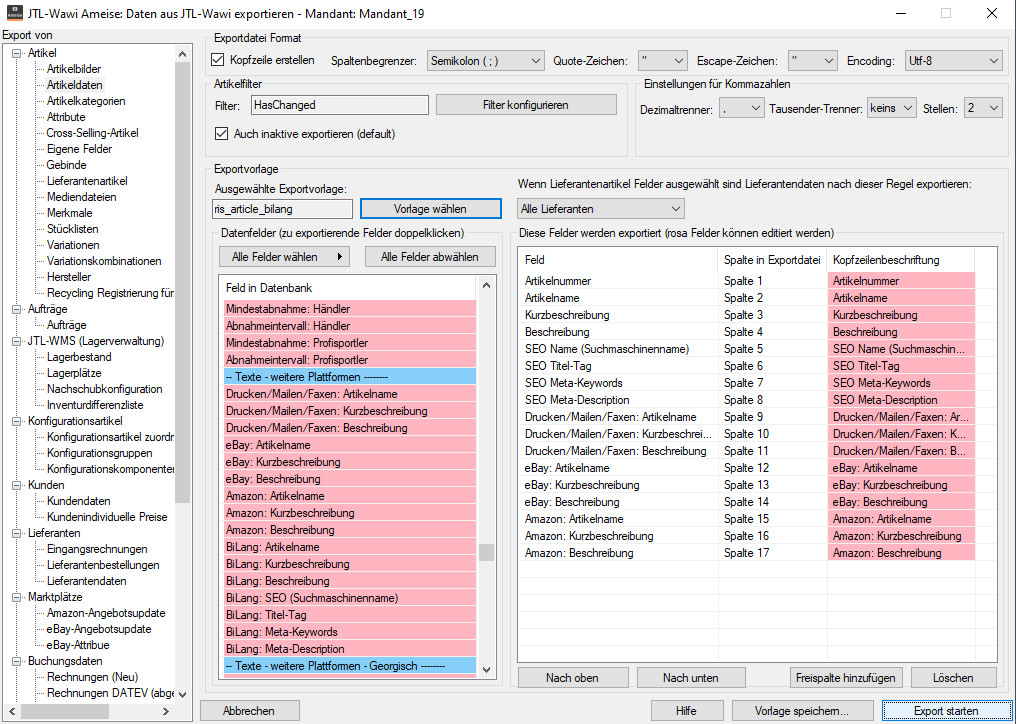
\includegraphics[width=15cm]{./img/AmeiseExport.png}

\newpage
\subsection{Konfigurationsdatei}
\label{sec:config}
\begin{lstlisting}[language=xml]
<?xml version="1.0" encoding="utf-8"?>
<configuration>
    <appSettings>
        <!-- connection to wawi db -->
        <add key="db_server" value="192.168.107.11\DEVWAWI" />
        <add key="db_mandant" value="Mandant_19" />
        <add key="db_pass" value="sa04jT14" />
        <add key="db_user" value="sa" />
        <add key="db_port" value="57981" />

        <!-- Ameisendaten -->
        <add key="jtlAmeisePath" value="C:\Programme\JTL-Software\JTL-wawi-ameise.exe" />
    </appSettings>

    <appLanguages>
        <!-- add key="BG" value="" -->
        <!-- add key="CS" value="" -->
        <!-- add key="DA" value="" -->
        <!-- add key="DE" value="" -->
        <!-- add key="EL" value="" -->
        <add key="EN" value="" />
        <!-- add key="ES" value="" -->
        <!-- add key="ET" value="" -->
        <!-- add key="FI" value="" -->
        <!-- add key="FR" value="" -->
        <!-- add key="HU" value="" -->
        <!-- add key="IT" value="" -->
        <!-- add key="JA" value="" -->
        <!-- add key="LT" value="" -->
        <!-- add key="LV" value="" -->
        <!-- add key="NL" value="" -->
        <!-- add key="PL" value="" -->
        <!-- add key="PT" value="" -->
        <!-- add key="RO" value="" -->
        <!-- add key="RU" value="" -->
        <!-- add key="SK" value="" -->
        <!-- add key="SL" value="" -->
        <!-- add key="SV" value="" -->
        <!-- add key="ZH" value="" -->
    </appLanguages>
</configuration>
\end{lstlisting}


\newpage
\subsection{SqlHelper}
\label{sec:sql_helper}
\begin{lstlisting}[language=php]
using System;
using System.Configuration;
using System.Data.SqlClient;

namespace Bilang.Classes {
    public class SqlHelper {
        public String DbServer { get; set; }
        public String Db { get; set; }
        public String DbUser { get; set; }
        public String DbPass { get; set; }
        public int DbPort { get; set; }
        private String connectionString =>
            "user id=" + DbUser + ";" +
            "password=" + DbPass +
            ";server=" + DbServer+ ((DbPort > 0) ? $",{DbPort}" : "") +
            ";Trusted_Connection=no;Connect Timeout=10;" +
            "Pooling=false;" +
            "database=" + Db + "; " +
            "connection timeout=30";

        public SqlHelper() {
            var config = ConfigurationManager.OpenExeConfiguration(ConfigurationUserLevel.None);
            DbServer = config.AppSettings.Settings["db_server"].Value.Trim();
            Db = config.AppSettings.Settings["db_mandant"].Value.Trim();
            DbUser = config.AppSettings.Settings["db_user"].Value.Trim();
            DbPass = config.AppSettings.Settings["db_pass"].Value.Trim();
            DbPort = int.Parse(config.AppSettings.Settings["db_port"].Value.Trim());
        }
        public void execute(String query) {
            using SqlConnection connection = new SqlConnection(connectionString);
            
            connection.Open();

            SqlCommand execute = new SqlCommand(query, connection);
            execute.ExecuteNonQuery();
            Console.WriteLine("Inserting Data Successfully");

            connection.Close();
        }
    }
}
\end{lstlisting}

\subsection{Tabelle 'hash'}
\label{sec:table_hash}
\begin{tabular}{ |l|l|l|l|l| }
	\hline
	ID & object\_type & object\_id & hash \\ 
	\hline
	\dots & \dots & \dots & \dots\\  
	255 & kArtikel & 45621 & e3b0c44298fc1c149\dots\\  
	256 & kArtikel & 45621 & 9f86d081884c7d659\dots\\  
	257 & kKategorie & 19017 & 34ca495991b7852b8\dots\\  
	\dots & \dots & \dots & \dots\\  
	\hline
\end{tabular}

\subsection{Tabelle 'hash\_language'}
\label{sec:table_hash_language}
\begin{tabular}{ |l|l|l|l|l| }
	\hline
	ID & hash\_id & language\_iso \\ 
	\hline
	\dots & \dots & \dots \\  
	419 & 255 & EN\\  
	420 & 255 & NL\\  
	410 & 256 & EN\\  
	\dots & \dots & \dots \\  
	\hline
\end{tabular}

\newpage
\subsection{ApiHelper}
\label{sec:api_helper}
\begin{lstlisting}[language=php]
public static string PostRequest(string url, string payload) {

    HttpWebRequest request = (HttpWebRequest)WebRequest.Create(url);
    request.Method = "POST";
    request.ContentType = "application/json";

    using(var streamWriter = new StreamWriter(request.GetRequestStream())) {
        streamWriter.Write(payload);
    }

    HttpWebResponse response = null;
    string responseStr = "";

    try {
        response = (HttpWebResponse)request.GetResponse();
        responseStr = ReadAllFromResponse(response);
    }
    catch(WebException e) {
        Console.Write("---\tError in request:\n" + e + "\n---");
    }

    using(var streamReader = new StreamReader(response.GetResponseStream())) {
        var result = streamReader.ReadToEnd();
    }

    return responseStr;
}
\end{lstlisting}

\subsection{Weichstelle der API für Tests}
\label{sec:testing_api}
\begin{lstlisting}[language=php]
if($data['api_key'] == "9876543210"){
    return $data['destination_language_iso']."(".$data['content'].")";
}
\end{lstlisting}
\newpage
% !TEX root = Projektdokumentation.tex
\section{Benutzerhandbuch}
\label{sec:api_documentation}
\vspace*{36 pt}
\vspace{4cm}
\begin{center}\Huge\bfseries\itshape
BiLang-API: \\
Technische Dokumentation
\end{center}	

\vspace{11cm}
\begin{center}\large
	Version 1.0.0 vom 19.05.2021 \\
	Autor: \companyName
\end{center}
\newpage


Dies ist eine technische Dokumentation für die BiLang-Übersetzungs-API. 
Sie ist die Schnittstelle für die beiden anderen Komponenten der BiLang-Software. 
Sowohl das JTL-Shop-Plugin als auch die Zusatzsoftware für die JTL-Wawi sind auf diese API angewiesen. 

Eine Anfrage an die API besteht grundsätzlich immer folgenden 4 Parametern:

\begin{tabular}{ |l|l| }
	\hline
	Parameter & Beschreibung \\
	\hline
	content & Zu Übersetzender Text. \\
	\hline
	source\_language\_iso & Ausgangssprache des Parameters 'content'. \\
	 & \(\cdot\) 'CS' - Tschechisch \\
	 & \(\cdot\) 'DE' - Deutsch \\
	 & \(\cdot\) 'EL' - Griechisch \\
	 & \(\cdot\) 'EN' - Englisch \\
	 & \(\cdot\) 'ES' - Spanisch \\
	 & \(\cdot\) 'FR' - Französisch \\
	 & \(\cdot\) 'HU' - Ungarisch \\
	 & \(\cdot\) 'IT' - Italienisch \\
	 & \(\cdot\) 'NL' - Niederländisch \\
	 & \(\cdot\) 'PL' - Polnisch \\
	 & \(\cdot\) 'PT' - Portugiesisch \\
	 & \(\cdot\) 'RU' - Russisch \\
	 & \(\cdot\) 'SV' - Schwedisch \\
	 \hline
	destination\_language\_iso & Zielsprache in die 'content' übersetzt werden soll. \\
	 & \(\cdot\) 'CS' - Tschechisch \\
	 & \(\cdot\) 'DE' - Deutsch \\
	 & \(\cdot\) 'EL' - Griechisch \\
	 & \(\cdot\) 'EN' - Englisch \\
	 & \(\cdot\) 'ES' - Spanisch \\
	 & \(\cdot\) 'FR' - Französisch \\
	 & \(\cdot\) 'HU' - Ungarisch \\
	 & \(\cdot\) 'IT' - Italienisch \\
	 & \(\cdot\) 'NL' - Niederländisch \\
	 & \(\cdot\) 'PL' - Polnisch \\
	 & \(\cdot\) 'PT' - Portugiesisch \\
	 & \(\cdot\) 'RU' - Russisch \\
	 & \(\cdot\) 'SV' - Schwedisch \\
	 \hline
	api\_key & Bei Vertragsschluss wird Ihnen ein API-Key übergeben. \\
	 & Bei Fragen wenden Sie sich bitte an den {\href{mailto:support@ris-development.de}{Support}}. \\
	\hline
\end{tabular}


Dabei kann 'content' auch Inhalte mit XML-Format beinhalten, die XML-Tags werden dann nicht mit übersetzt, 
um HTML-Strukturen wie zum Beispiel Attribute oder Anker korrekt beizubehalten.

\paragraph{Beispiele}

HTTP-Methode: POST auf bilang.ris-development.net/translation\_request
\begin{lstlisting}[extendedchars=\true,]
	{
		"content": "bÜersetzung", 
		"source_language_iso": "DE", 
		"destination_language_iso": "EN",
		"api_key": "9876543210"
	}
\end{lstlisting}


Response:
\begin{lstlisting}[extendedchars=\true,]
	Translation
\end{lstlisting}

 \vspace{2cm}

HTTP-Methode: POST auf bilang.ris-development.net/translation\_request
\begin{lstlisting}[extendedchars=\true,]
	{
		"content": "<a href="/büersetzung"> Übersetzung </a>",
		"source_language_iso": "DE",
		"destination_language_iso": "EN",
		"api_key": "9876543210"
	}
\end{lstlisting}

Response:
\begin{lstlisting}[extendedchars=\true,]
	<a href="/büersetzung"> Translation </a>
\end{lstlisting}

\paragraph{Limit}
Die maximale Anfragengröße darf 30kbytes nicht überschreiten, 

\paragraph{Formate und Sicherheit}
Die Parameter werden benutzt, um Informationen an die API zu übergeben. 
Dabei wird vorausgesetzt, dass alle Parameter den UTF8-Zeichensatz benutzen.
Die Antworten sind ebenfalls im UTF8-Zeichensatz.
Ihr API-Key ist absolut einmalig und wird bei jeder Anfrage überprüft.
Der gesamte Datenaustausch wird mit SSL abgesichert.
\newpage
% !TEX root = Projektdokumentation.tex
\section{Installationsanleitung}

\label{sec:tool_documentation}
\vspace*{36 pt}
\vspace{4cm}
\begin{center}\Huge\bfseries\itshape
BiLang-Zusatzsoftware: Installationsanleitung
\end{center}	

\vspace{11cm}
\begin{center}\large
	Version 1.0.0 vom 19.05.2021 \\
	Autor: \companyName
\end{center}

\newpage

\paragraph{1. Einleitung:}

Um eine Installation erfolgreich abzuschließen, befolgen Sie bitte sämtliche Schritte, die in dieser Anleitung anschaulich erklärt werden. Sie benötigen:

\begin{itemize}
	\item Zugangs- und Installationsrechte auf dem Windowssystem
	\item Zugangsdaten zu einem JTL-Wawi-Benutzer mit entsprechend hohen Rechten.
	\item Zugangsdaten zur JTL-Wawi-Datenbank
	\item Einen gültigen API-Schlüssel
	\item Die Software in der aktuellen Version zusammen mit den Ex- und Importvorlagen
\end{itemize}

\paragraph{2. Vorbereiten der Installation:}
Transferieren Sie die Software auf das Windowssystem auf dem auch die JTL-Wawi-Datenbank aktiv läuft.

\paragraph{3. Eigenes Feld anlegen:}
\begin{itemize}
	\item Erstellen Sie ein 'Eigenes Feld' das als Indentikator benutzt dafür verwerden werden kann, ob ein Artikel sich verändert hat oder nicht. 
	\item Wählen Sie dazu zuerst den Menüpunkt 'Admin -> Eigene Felder'.
	\item Legen Sie nun die 'RIS\_BiLang' Feldgruppe an, in der das Feld 'ArticleChanged' eingetragen wird. 
	\item Sie können außerdem unten links auswählen welche Warengruppen Sie übersetzen lassen möchten.
	\item Das Feld muss vom Datentyp 'Checkbox' sein, Anzeigeort und Beschreibung können frei gewählt werden.
	\item Bestätigen Sie Ihre Angaben, indem Sie die 'Speichern' Schaltfläche benutzen.
\end{itemize}

\begin{center}
	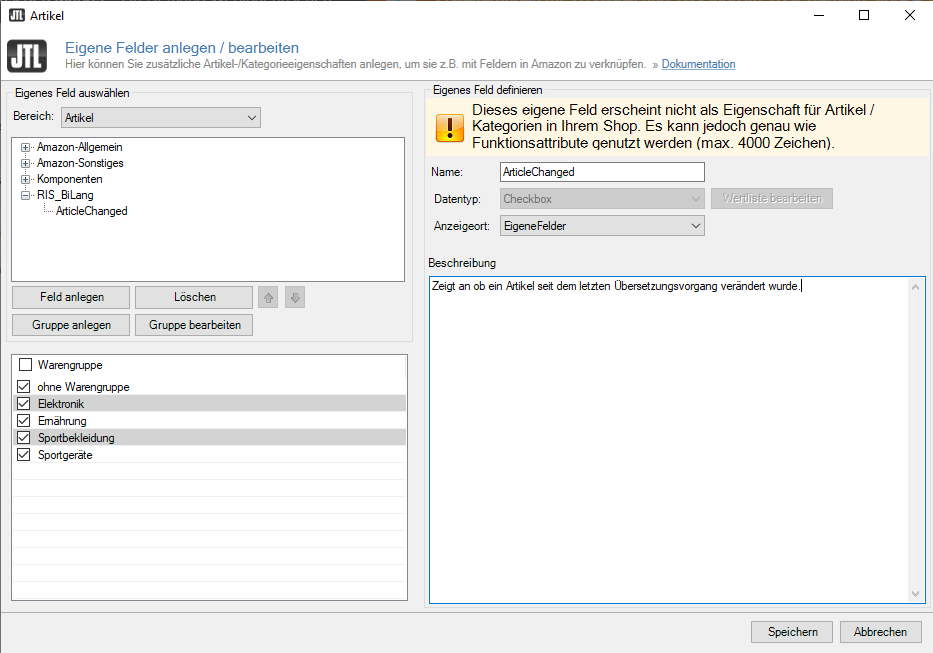
\includegraphics[width=9cm]{./img/eigenesFeld.png}
\end{center}

\paragraph{4. JTL-Wawi Workflow anlegen:}
Nun muss das soeben erstellte Feld benutzt werden, dazu wählen Sie wieder 'Admin' und nun 'JTL-Workflows':

\begin{itemize}
	\item Da das Feld immer dann auf Wahr gesetzt werden soll, wenn ein Artikel sich verändert hat, wird ein Workflow für das Ereignis 'Artikel - Geändert' erstellt.
	\item Die Bedingung kann verändert werden, es wird allerdings empfohlen keine Bedingung anzugeben.
	\item Erstellen Sie eine neue Aktion, indem Sie auf den entsprechenden Text klicken.
	\item Im Dropdown Menü wird die Option 'Werte setzen' ausgewählt und anschließend das 'ArticleChanged' als Variable gewählt.
	\item Bestätigen Sie Ihre Angaben, indem Sie die 'Speichern' Schaltfläche benutzen.
\end{itemize}
	
\begin{center}
	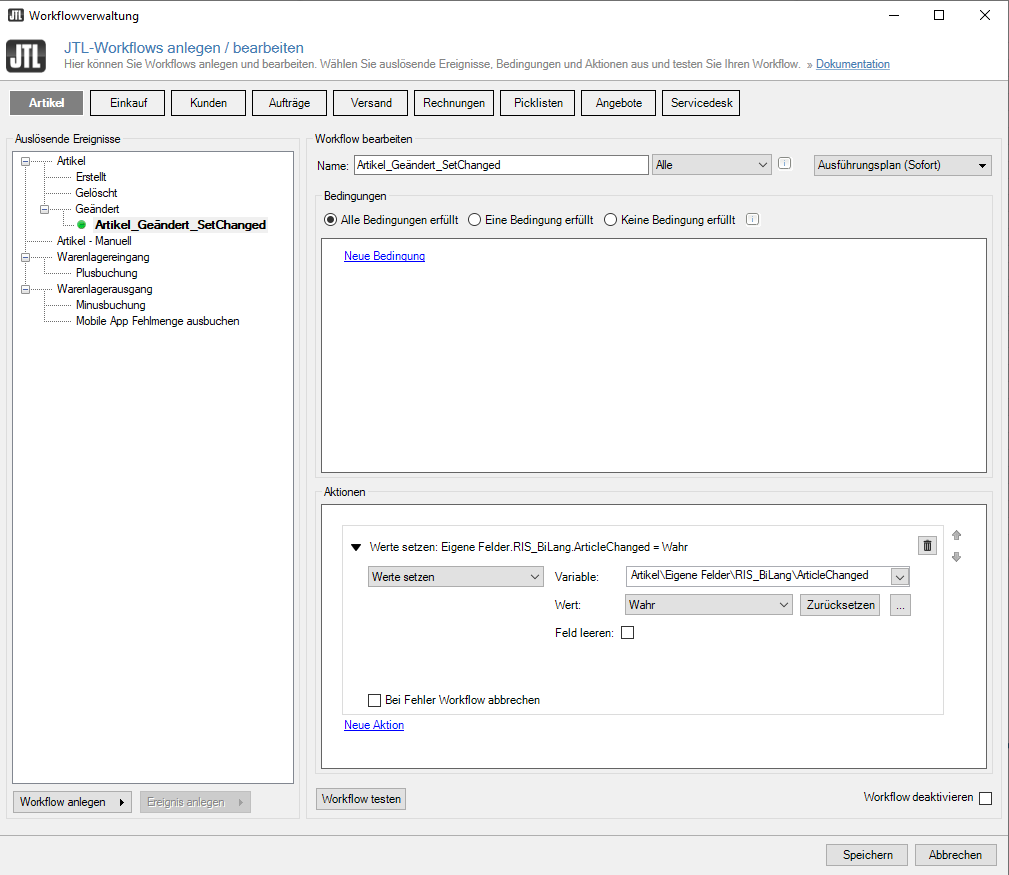
\includegraphics[width=9cm]{./img/workflows.png}
\end{center}

\paragraph{5. Konfigurationsdatei anpassen:}
Damit das Programm eine Verbindung zum JTL-Wawi Datenbankserver herstellen kann, muss die Konfigurationsdatei richtig beschrieben werden.
Im Bereich \texttt{appSettings} finden Sie verschiedene Punkte. 

\texttt{db\_server} : Die IP-Adresse des Datenbankservers mit der Instanz der JTL-Wawi-Datenbank als Anhang, getrennt durch einen ``\textbackslash''.

\texttt{db\_port} : Der Port unter dem die Datenbank angesprochen werden kann.

\texttt{db\_mandant} : Der Name des Mandanten für den die Übersetzung aktiviert werden soll.

\texttt{db\_user} : Der Benutzername zu einem Datenbankbenutzer (Standardwert 'sa').

\texttt{db\_pass} : Das Passwort zum Datenbankbenutzername in db\_user (Standardwert 'sa04jT14').

\texttt{jtlAmeisePath} : Der absolute Pfad zur 'JTL-wawi-ameise.exe', welche im Installationsverzeichnis liegt (Standardwert 'C:\textbackslash Programme\textbackslash JTL-Software\textbackslash JTL-wawi-ameise.exe').

Außerdem können die \texttt{appLanguages} nach Belieben ein- oder auskommentiert werden, um diese auch tatsächlich zu nutzen.

\paragraph{6. Windows-Aufgabenplanung konfigurieren:}%
Um das Programm automatisiert starten zu lassen, verwenden Sie die Windows-Aufgabenplanung. 
Diese ermöglicht Programmstarts mit festen Intervallen.

\begin{center}
	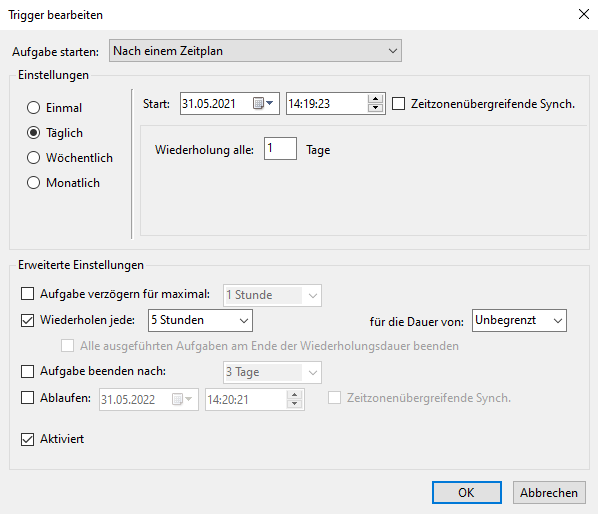
\includegraphics[width=9cm]{./img/Aufgabenplanung3.png}
\end{center}

\begin{itemize}
	\item Dazu müssen Sie eine 'Aufgabe erstellen...'
	\item Name und Beschreibung ist frei wählbar
	\item Wechseln Sie in den Reiter 'Trigger' und legen einen neuen Trigger an
\end{itemize}

\begin{center}
	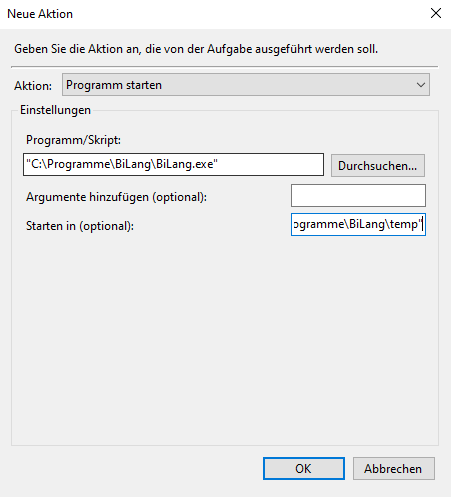
\includegraphics[width=8cm]{./img/Aufgabenplanung2.png}
\end{center}

\begin{itemize}
	\item Hier wird angegeben, wie oft das Programm eine Übersetzung anstoßen soll. Empfohlen wird eine Tägliche Ausführung, sowie manuelle Starts bei großen Veränderungen in den Stammdaten der JTL-Wawi.
	\item Nach eine Bestätigung mit OK, können Sie auf den Reiter 'Aktionen' wechseln. 
	\item Hier erstellen Sie eine neue Aktion vom Typ 'Programm starten' und wählen die BiLang.exe aus Ihrem Verzeichnis aus.
	\item Empfohlen wird in dem Feld 'Starten in' den absoluten Pfad des Verzeichnisses 'BiLang/temp' auszuwählen.
\end{itemize}
\newpage
\thispagestyle{empty}
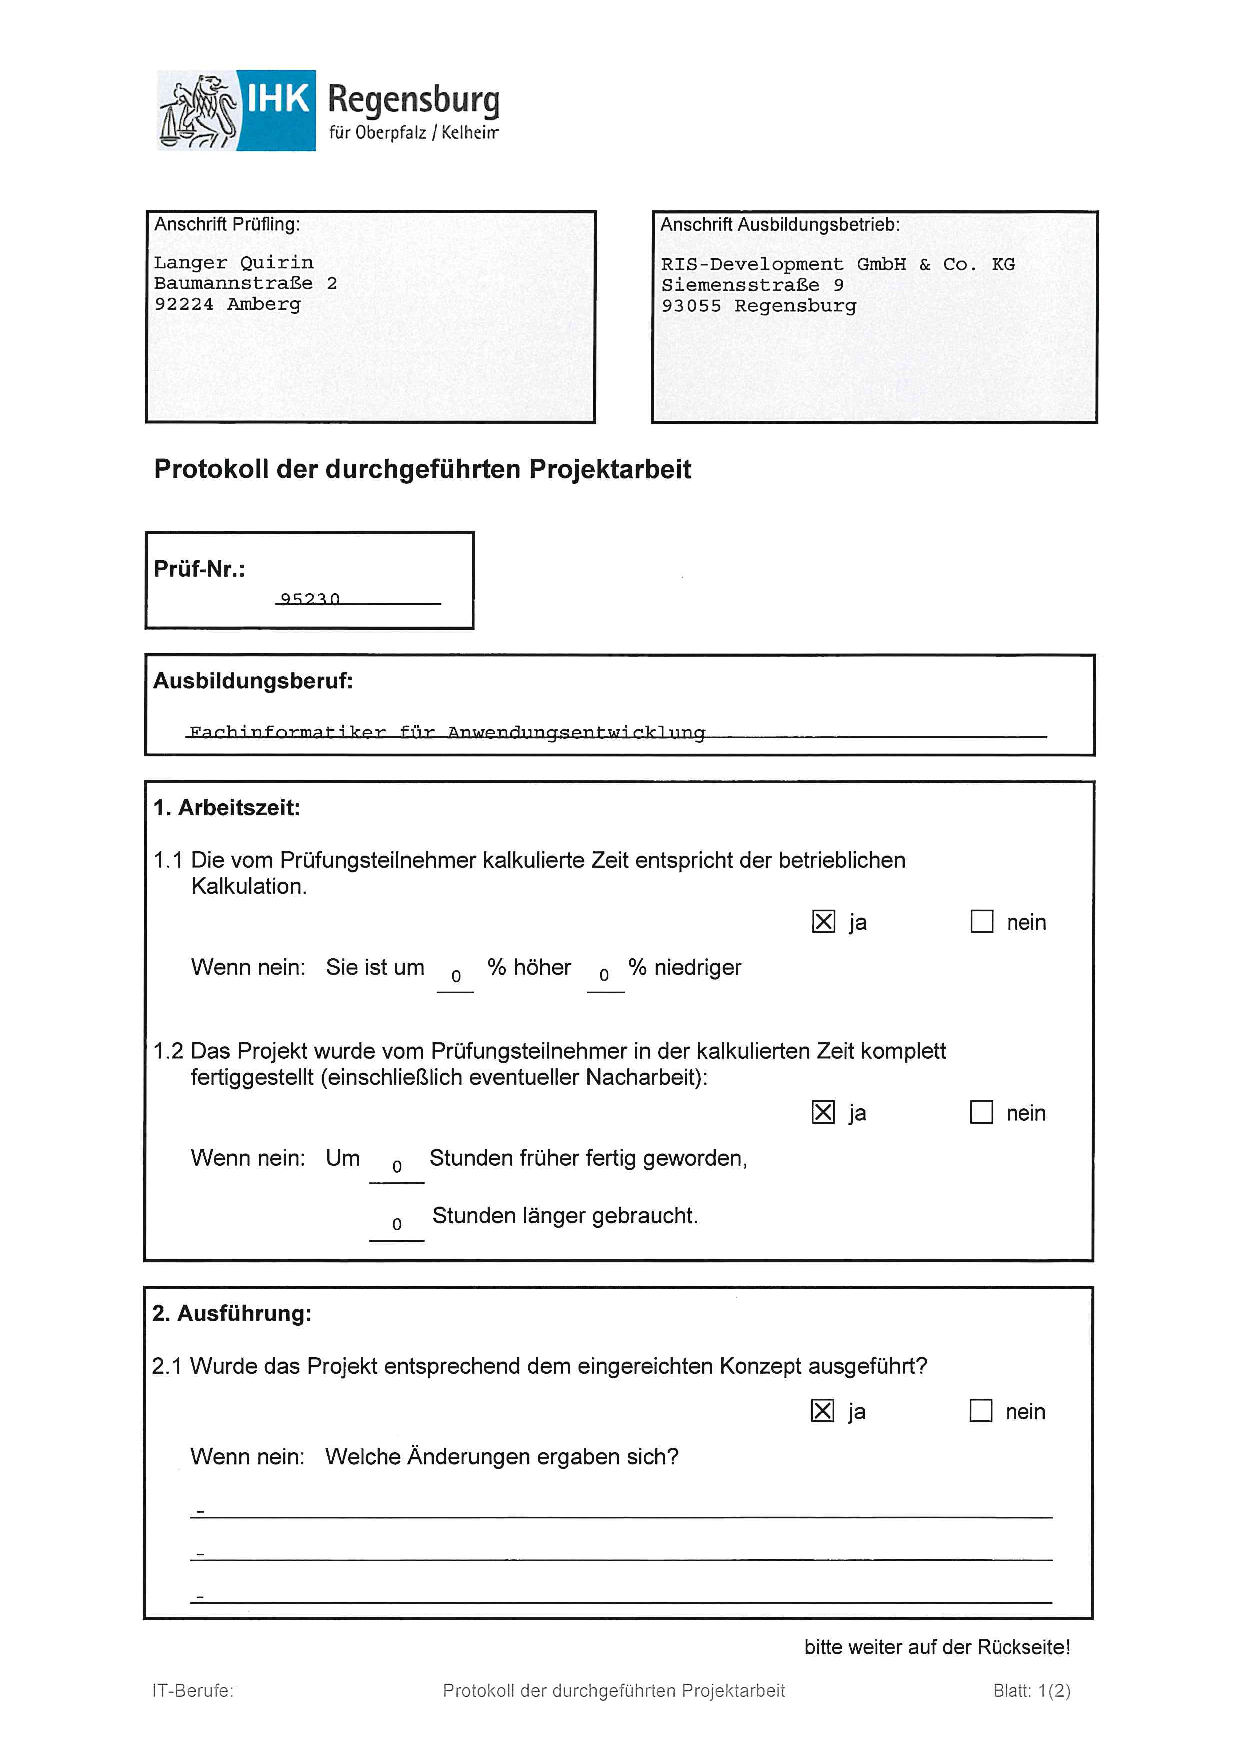
\includepdf[pages={1-}]{./ANHANG.pdf}
\end{document}
